\subsection{GPU: version using shared memory}
The task is split into different subtasks. For the first subtask, we measured the execution time of different threads-per-block, our chosen problem size is the size 2048 * 2048. The result shows that, with shared memory, the optimal execution time varies between the dimension of 8 on each block Size untill the range of 13 on the block size. With larger block sizes, using a problemsize of 2048*2048, the execution time worsens. This can also be seen in graphic \ref{fig:shared_vs_naive}.
\begin{figure}[h]
    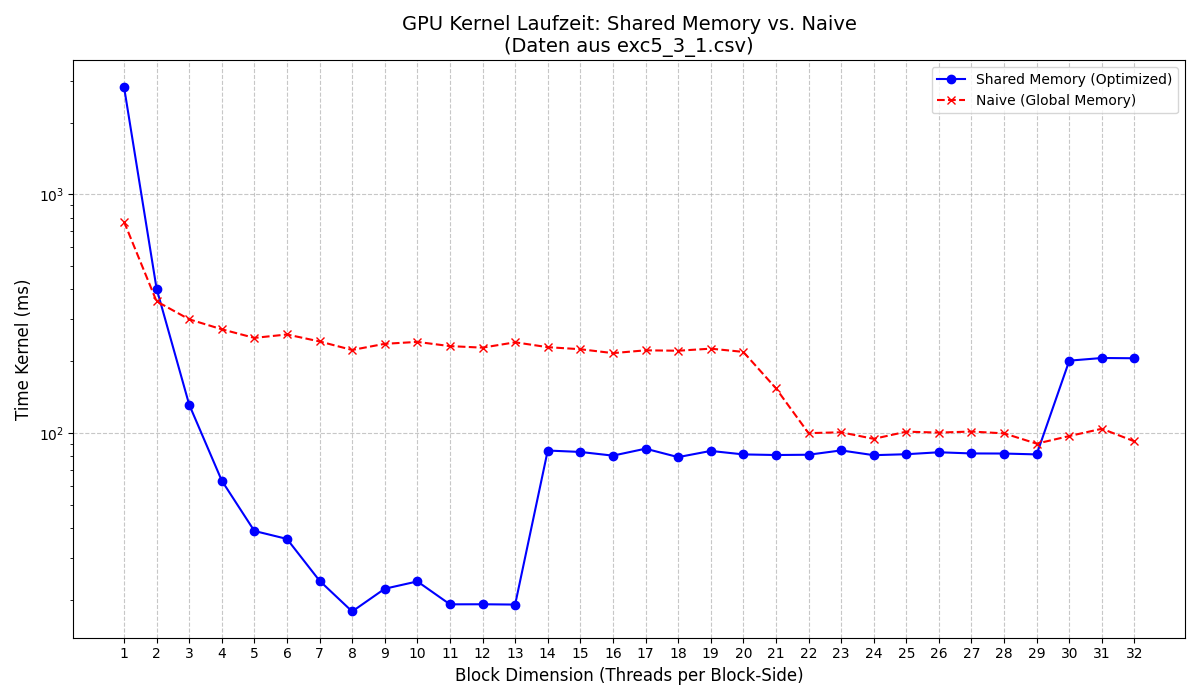
\includegraphics[width=\textwidth]{GPUKernelLaufzeitSharedMemoryVsNaive_2048_2048__LOG.png}
    \caption{Runtime in Shared Memory vs. Naive memory}
    \label{fig:shared_vs_naive}
\end{figure}
\\
The secound subtask explains the overall runtime together with different components over different problem sizes. It is visible, that with a larger problem size, the execution time increases as well. \ref{fig:shared_TOTAL} shows the steady increase in time. 
\begin{figure}[h]
    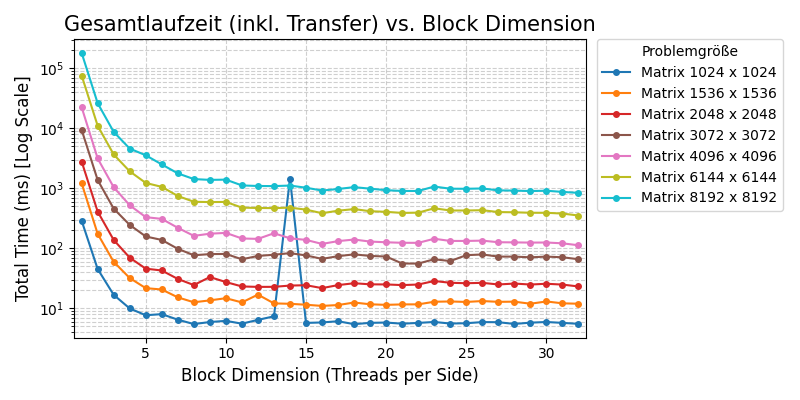
\includegraphics[width=\textwidth]{exc5_3_2_Vary_Threads_Diffrent_Problemsize.png}
    \caption{Executiontime of diffrent problemsizes by diffrent threads per Block}
    \label{fig:shared_TOTAL}
\end{figure}
The spike in the 1024 * 1024 matrix could be a loading error of the Cluster.
\\
In the last subtask of the section, the speedup from shared to naive execution is beeing explored. Hereby we explore with the Kernel Speedup the computing speedup only, and with APplicationSpeedup the overall time of the Whole programm with the H2D, D2H and Kernel time together. The chosen speedup we look at is the speeup by a blocksize of 32. A Maximum speedup faktor of 1.916 can be messured.
The results can be viewed in \ref{fig:speedup_TOTAL_2}.
\begin{figure}[h]
    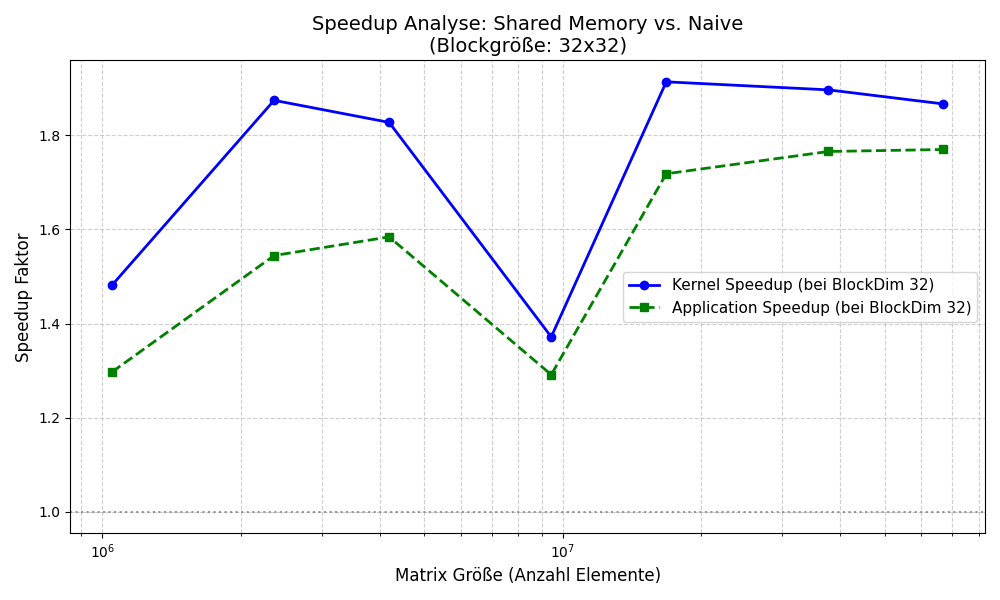
\includegraphics[width=\textwidth]{exc5_3_3_Speedup.png}
    \caption{Speedup of Kernel without and with enviroment}
    \label{fig:speedup_TOTAL_2}
\end{figure}